%% bare_jrnl_compsoc.tex
%% V1.4b
%% 2015/08/26
%% by Michael Shell
%% See:
%% http://www.michaelshell.org/
%% for current contact information.
%%
%% This is a skeleton file demonstrating the use of IEEEtran.cls
%% (requires IEEEtran.cls version 1.8b or later) with an IEEE
%% Computer Society journal paper.
%%
%% Support sites:
%% http://www.michaelshell.org/tex/ieeetran/
%% http://www.ctan.org/pkg/ieeetran
%% and
%% http://www.ieee.org/

%%*************************************************************************
%% Legal Notice:
%% This code is offered as-is without any warranty either expressed or
%% implied; without even the implied warranty of MERCHANTABILITY or
%% FITNESS FOR A PARTICULAR PURPOSE! 
%% User assumes all risk.
%% In no event shall the IEEE or any contributor to this code be liable for
%% any damages or losses, including, but not limited to, incidental,
%% consequential, or any other damages, resulting from the use or misuse
%% of any information contained here.
%%
%% All comments are the opinions of their respective authors and are not
%% necessarily endorsed by the IEEE.
%%
%% This work is distributed under the LaTeX Project Public License (LPPL)
%% ( http://www.latex-project.org/ ) version 1.3, and may be freely used,
%% distributed and modified. A copy of the LPPL, version 1.3, is included
%% in the base LaTeX documentation of all distributions of LaTeX released
%% 2003/12/01 or later.
%% Retain all contribution notices and credits.
%% ** Modified files should be clearly indicated as such, including  **
%% ** renaming them and changing author support contact information. **
%%*************************************************************************


% *** Authors should verify (and, if needed, correct) their LaTeX system  ***
% *** with the testflow diagnostic prior to trusting their LaTeX platform ***
% *** with production work. The IEEE's font choices and paper sizes can   ***
% *** trigger bugs that do not appear when using other class files.       ***                          ***
% The testflow support page is at:
% http://www.michaelshell.org/tex/testflow/


\documentclass[10pt,journal,compsoc]{IEEEtran}
%
% If IEEEtran.cls has not been installed into the LaTeX system files,
% manually specify the path to it like:
% \documentclass[10pt,journal,compsoc]{../sty/IEEEtran}





% Some very useful LaTeX packages include:
% (uncomment the ones you want to load)


% *** MISC UTILITY PACKAGES ***
%
%\usepackage{ifpdf}
% Heiko Oberdiek's ifpdf.sty is very useful if you need conditional
% compilation based on whether the output is pdf or dvi.
% usage:
% \ifpdf
%   % pdf code
% \else
%   % dvi code
% \fi
% The latest version of ifpdf.sty can be obtained from:
% http://www.ctan.org/pkg/ifpdf
% Also, note that IEEEtran.cls V1.7 and later provides a builtin
% \ifCLASSINFOpdf conditional that works the same way.
% When switching from latex to pdflatex and vice-versa, the compiler may
% have to be run twice to clear warning/error messages.






% *** CITATION PACKAGES ***
%
\ifCLASSOPTIONcompsoc
  % IEEE Computer Society needs nocompress option
  % requires cite.sty v4.0 or later (November 2003)
  \usepackage[nocompress]{cite}
\else
  % normal IEEE
  \usepackage{cite}
\fi
% cite.sty was written by Donald Arseneau
% V1.6 and later of IEEEtran pre-defines the format of the cite.sty package
% \cite{} output to follow that of the IEEE. Loading the cite package will
% result in citation numbers being automatically sorted and properly
% "compressed/ranged". e.g., [1], [9], [2], [7], [5], [6] without using
% cite.sty will become [1], [2], [5]--[7], [9] using cite.sty. cite.sty's
% \cite will automatically add leading space, if needed. Use cite.sty's
% noadjust option (cite.sty V3.8 and later) if you want to turn this off
% such as if a citation ever needs to be enclosed in parenthesis.
% cite.sty is already installed on most LaTeX systems. Be sure and use
% version 5.0 (2009-03-20) and later if using hyperref.sty.
% The latest version can be obtained at:
% http://www.ctan.org/pkg/cite
% The documentation is contained in the cite.sty file itself.
%
% Note that some packages require special options to format as the Computer
% Society requires. In particular, Computer Society  papers do not use
% compressed citation ranges as is done in typical IEEE papers
% (e.g., [1]-[4]). Instead, they list every citation separately in order
% (e.g., [1], [2], [3], [4]). To get the latter we need to load the cite
% package with the nocompress option which is supported by cite.sty v4.0
% and later. Note also the use of a CLASSOPTION conditional provided by
% IEEEtran.cls V1.7 and later.





% *** GRAPHICS RELATED PACKAGES ***
%
\ifCLASSINFOpdf
  % \usepackage[pdftex]{graphicx}
  % declare the path(s) where your graphic files are
  % \graphicspath{{../pdf/}{../jpeg/}}
  % and their extensions so you won't have to specify these with
  % every instance of \includegraphics
  % \DeclareGraphicsExtensions{.pdf,.jpeg,.png}
\else
  % or other class option (dvipsone, dvipdf, if not using dvips). graphicx
  % will default to the driver specified in the system graphics.cfg if no
  % driver is specified.
  % \usepackage[dvips]{graphicx}
  % declare the path(s) where your graphic files are
  % \graphicspath{{../eps/}}
  % and their extensions so you won't have to specify these with
  % every instance of \includegraphics
  % \DeclareGraphicsExtensions{.eps}
\fi
% graphicx was written by David Carlisle and Sebastian Rahtz. It is
% required if you want graphics, photos, etc. graphicx.sty is already
% installed on most LaTeX systems. The latest version and documentation
% can be obtained at: 
% http://www.ctan.org/pkg/graphicx
% Another good source of documentation is "Using Imported Graphics in
% LaTeX2e" by Keith Reckdahl which can be found at:
% http://www.ctan.org/pkg/epslatex
%
% latex, and pdflatex in dvi mode, support graphics in encapsulated
% postscript (.eps) format. pdflatex in pdf mode supports graphics
% in .pdf, .jpeg, .png and .mps (metapost) formats. Users should ensure
% that all non-photo figures use a vector format (.eps, .pdf, .mps) and
% not a bitmapped formats (.jpeg, .png). The IEEE frowns on bitmapped formats
% which can result in "jaggedy"/blurry rendering of lines and letters as
% well as large increases in file sizes.
%
% You can find documentation about the pdfTeX application at:
% http://www.tug.org/applications/pdftex






% *** MATH PACKAGES ***
%
\usepackage{amsmath}
\usepackage{amsfonts}
% A popular package from the American Mathematical Society that provides
% many useful and powerful commands for dealing with mathematics.
%
% Note that the amsmath package sets \interdisplaylinepenalty to 10000
% thus preventing page breaks from occurring within multiline equations. Use:
%\interdisplaylinepenalty=2500
% after loading amsmath to restore such page breaks as IEEEtran.cls normally
% does. amsmath.sty is already installed on most LaTeX systems. The latest
% version and documentation can be obtained at:
% http://www.ctan.org/pkg/amsmath





% *** SPECIALIZED LIST PACKAGES ***
%
%\usepackage{algorithmic}
% algorithmic.sty was written by Peter Williams and Rogerio Brito.
% This package provides an algorithmic environment fo describing algorithms.
% You can use the algorithmic environment in-text or within a figure
% environment to provide for a floating algorithm. Do NOT use the algorithm
% floating environment provided by algorithm.sty (by the same authors) or
% algorithm2e.sty (by Christophe Fiorio) as the IEEE does not use dedicated
% algorithm float types and packages that provide these will not provide
% correct IEEE style captions. The latest version and documentation of
% algorithmic.sty can be obtained at:
% http://www.ctan.org/pkg/algorithms
% Also of interest may be the (relatively newer and more customizable)
% algorithmicx.sty package by Szasz Janos:
% http://www.ctan.org/pkg/algorithmicx




% *** ALIGNMENT PACKAGES ***
%
%\usepackage{array}
% Frank Mittelbach's and David Carlisle's array.sty patches and improves
% the standard LaTeX2e array and tabular environments to provide better
% appearance and additional user controls. As the default LaTeX2e table
% generation code is lacking to the point of almost being broken with
% respect to the quality of the end results, all users are strongly
% advised to use an enhanced (at the very least that provided by array.sty)
% set of table tools. array.sty is already installed on most systems. The
% latest version and documentation can be obtained at:
% http://www.ctan.org/pkg/array


% IEEEtran contains the IEEEeqnarray family of commands that can be used to
% generate multiline equations as well as matrices, tables, etc., of high
% quality.




% *** SUBFIGURE PACKAGES ***
\ifCLASSOPTIONcompsoc
 \usepackage[caption=false,font=footnotesize,labelfont=sf,textfont=sf]{subfig}
\else
 \usepackage[caption=false,font=footnotesize]{subfig}
\fi
% subfig.sty, written by Steven Douglas Cochran, is the modern replacement
% for subfigure.sty, the latter of which is no longer maintained and is
% incompatible with some LaTeX packages including fixltx2e. However,
% subfig.sty requires and automatically loads Axel Sommerfeldt's caption.sty
% which will override IEEEtran.cls' handling of captions and this will result
% in non-IEEE style figure/table captions. To prevent this problem, be sure
% and invoke subfig.sty's "caption=false" package option (available since
% subfig.sty version 1.3, 2005/06/28) as this is will preserve IEEEtran.cls
% handling of captions.
% Note that the Computer Society format requires a sans serif font rather
% than the serif font used in traditional IEEE formatting and thus the need
% to invoke different subfig.sty package options depending on whether
% compsoc mode has been enabled.
%
% The latest version and documentation of subfig.sty can be obtained at:
% http://www.ctan.org/pkg/subfig




% *** FLOAT PACKAGES ***
%
%\usepackage{fixltx2e}
% fixltx2e, the successor to the earlier fix2col.sty, was written by
% Frank Mittelbach and David Carlisle. This package corrects a few problems
% in the LaTeX2e kernel, the most notable of which is that in current
% LaTeX2e releases, the ordering of single and double column floats is not
% guaranteed to be preserved. Thus, an unpatched LaTeX2e can allow a
% single column figure to be placed prior to an earlier double column
% figure.
% Be aware that LaTeX2e kernels dated 2015 and later have fixltx2e.sty's
% corrections already built into the system in which case a warning will
% be issued if an attempt is made to load fixltx2e.sty as it is no longer
% needed.
% The latest version and documentation can be found at:
% http://www.ctan.org/pkg/fixltx2e


\usepackage{stfloats}
% stfloats.sty was written by Sigitas Tolusis. This package gives LaTeX2e
% the ability to do double column floats at the bottom of the page as well
% as the top. (e.g., "\begin{figure*}[!b]" is not normally possible in
% LaTeX2e). It also provides a command:
%\fnbelowfloat
% to enable the placement of footnotes below bottom floats (the standard
% LaTeX2e kernel puts them above bottom floats). This is an invasive package
% which rewrites many portions of the LaTeX2e float routines. It may not work
% with other packages that modify the LaTeX2e float routines. The latest
% version and documentation can be obtained at:
% http://www.ctan.org/pkg/stfloats
% Do not use the stfloats baselinefloat ability as the IEEE does not allow
% \baselineskip to stretch. Authors submitting work to the IEEE should note
% that the IEEE rarely uses double column equations and that authors should try
% to avoid such use. Do not be tempted to use the cuted.sty or midfloat.sty
% packages (also by Sigitas Tolusis) as the IEEE does not format its papers in
% such ways.
% Do not attempt to use stfloats with fixltx2e as they are incompatible.
% Instead, use Morten Hogholm'a dblfloatfix which combines the features
% of both fixltx2e and stfloats:
%
% \usepackage{dblfloatfix}
% The latest version can be found at:
% http://www.ctan.org/pkg/dblfloatfix




%\ifCLASSOPTIONcaptionsoff
%  \usepackage[nomarkers]{endfloat}
% \let\MYoriglatexcaption\caption
% \renewcommand{\caption}[2][\relax]{\MYoriglatexcaption[#2]{#2}}
%\fi
% endfloat.sty was written by James Darrell McCauley, Jeff Goldberg and 
% Axel Sommerfeldt. This package may be useful when used in conjunction with 
% IEEEtran.cls'  captionsoff option. Some IEEE journals/societies require that
% submissions have lists of figures/tables at the end of the paper and that
% figures/tables without any captions are placed on a page by themselves at
% the end of the document. If needed, the draftcls IEEEtran class option or
% \CLASSINPUTbaselinestretch interface can be used to increase the line
% spacing as well. Be sure and use the nomarkers option of endfloat to
% prevent endfloat from "marking" where the figures would have been placed
% in the text. The two hack lines of code above are a slight modification of
% that suggested by in the endfloat docs (section 8.4.1) to ensure that
% the full captions always appear in the list of figures/tables - even if
% the user used the short optional argument of \caption[]{}.
% IEEE papers do not typically make use of \caption[]'s optional argument,
% so this should not be an issue. A similar trick can be used to disable
% captions of packages such as subfig.sty that lack options to turn off
% the subcaptions:
% For subfig.sty:
% \let\MYorigsubfloat\subfloat
% \renewcommand{\subfloat}[2][\relax]{\MYorigsubfloat[]{#2}}
% However, the above trick will not work if both optional arguments of
% the \subfloat command are used. Furthermore, there needs to be a
% description of each subfigure *somewhere* and endfloat does not add
% subfigure captions to its list of figures. Thus, the best approach is to
% avoid the use of subfigure captions (many IEEE journals avoid them anyway)
% and instead reference/explain all the subfigures within the main caption.
% The latest version of endfloat.sty and its documentation can obtained at:
% http://www.ctan.org/pkg/endfloat
%
% The IEEEtran \ifCLASSOPTIONcaptionsoff conditional can also be used
% later in the document, say, to conditionally put the References on a 
% page by themselves.




% *** PDF, URL AND HYPERLINK PACKAGES ***
%
\usepackage{url}
% url.sty was written by Donald Arseneau. It provides better support for
% handling and breaking URLs. url.sty is already installed on most LaTeX
% systems. The latest version and documentation can be obtained at:
% http://www.ctan.org/pkg/url
% Basically, \url{my_url_here}.





% *** Do not adjust lengths that control margins, column widths, etc. ***
% *** Do not use packages that alter fonts (such as pslatex).         ***
% There should be no need to do such things with IEEEtran.cls V1.6 and later.
% (Unless specifically asked to do so by the journal or conference you plan
% to submit to, of course. )


% correct bad hyphenation here
\hyphenation{op-tical net-works semi-conduc-tor}

%
% paper title
% Titles are generally capitalized except for words such as a, an, and, as,
% at, but, by, for, in, nor, of, on, or, the, to and up, which are usually
% not capitalized unless they are the first or last word of the title.
% Linebreaks \\ can be used within to get better formatting as desired.
% Do not put math or special symbols in the title.

\title{One Model that Fits Them All: Psychometrics with Generalized Linear Mixed Effects Models}
%
%
% author names and IEEE memberships
% note positions of commas and nonbreaking spaces ( ~ ) LaTeX will not break
% a structure at a ~ so this keeps an author's name from being broken across
% two lines.
% use \thanks{} to gain access to the first footnote area
% a separate \thanks must be used for each paragraph as LaTeX2e's \thanks
% was not built to handle multiple paragraphs
%
%
%\IEEEcompsocitemizethanks is a special \thanks that produces the bulleted
% lists the Computer Society journals use for "first footnote" author
% affiliations. Use \IEEEcompsocthanksitem which works much like \item
% for each affiliation group. When not in compsoc mode,
% \IEEEcompsocitemizethanks becomes like \thanks and
% \IEEEcompsocthanksitem becomes a line break with idention. This
% facilitates dual compilation, although admittedly the differences in the
% desired content of \author between the different types of papers makes a
% one-size-fits-all approach a daunting prospect. For instance, compsoc 
% journal papers have the author affiliations above the "Manuscript
% received ..."  text while in non-compsoc journals this is reversed. Sigh.

\author{Wangqian~Ju,
        Susan~R~VanderPlas,
        and~Heike~Hofmann,% <-this % stops a space
\IEEEcompsocitemizethanks{\IEEEcompsocthanksitem W.\ Ju and H.\ Hofmann are with the Department
of Statistics, Iowa State University, Ames,
IA, 50010.\protect\\
% note need leading \protect in front of \\ to get a newline within \thanks as
% \\ is fragile and will error, could use \hfil\break instead.
E-mail: see http://www.michaelshell.org/contact.html
\IEEEcompsocthanksitem S.\ VanderPlas is with the Department of Statistics, University of Nebraska Lincoln.}% <-this % stops an unwanted space
\thanks{Manuscript received Month DD, YYYY; revised Month DD, YYYY.}}

% note the % following the last \IEEEmembership and also \thanks - 
% these prevent an unwanted space from occurring between the last author name
% and the end of the author line. i.e., if you had this:
% 
% \author{....lastname \thanks{...} \thanks{...} }
%                     ^------------^------------^----Do not want these spaces!
%
% a space would be appended to the last name and could cause every name on that
% line to be shifted left slightly. This is one of those "LaTeX things". For
% instance, "\textbf{A} \textbf{B}" will typeset as "A B" not "AB". To get
% "AB" then you have to do: "\textbf{A}\textbf{B}"
% \thanks is no different in this regard, so shield the last } of each \thanks
% that ends a line with a % and do not let a space in before the next \thanks.
% Spaces after \IEEEmembership other than the last one are OK (and needed) as
% you are supposed to have spaces between the names. For what it is worth,
% this is a minor point as most people would not even notice if the said evil
% space somehow managed to creep in.



% The paper headers
\markboth{Journal of \LaTeX\ Class Files,~Vol.~14, No.~8, August~2015}%
{Ju \MakeLowercase{\textit{et al.}}: Beyond Rasch }
% The only time the second header will appear is for the odd numbered pages
% after the title page when using the twoside option.
% 
% *** Note that you probably will NOT want to include the author's ***
% *** name in the headers of peer review papers.                   ***
% You can use \ifCLASSOPTIONpeerreview for conditional compilation here if
% you desire.



% The publisher's ID mark at the bottom of the page is less important with
% Computer Society journal papers as those publications place the marks
% outside of the main text columns and, therefore, unlike regular IEEE
% journals, the available text space is not reduced by their presence.
% If you want to put a publisher's ID mark on the page you can do it like
% this:
%\IEEEpubid{0000--0000/00\$00.00~\copyright~2015 IEEE}
% or like this to get the Computer Society new two part style.
%\IEEEpubid{\makebox[\columnwidth]{\hfill 0000--0000/00/\$00.00~\copyright~2015 IEEE}%
%\hspace{\columnsep}\makebox[\columnwidth]{Published by the IEEE Computer Society\hfill}}
% Remember, if you use this you must call \IEEEpubidadjcol in the second
% column for its text to clear the IEEEpubid mark (Computer Society jorunal
% papers don't need this extra clearance.)



% use for special paper notices
%\IEEEspecialpapernotice{(Invited Paper)}



% for Computer Society papers, we must declare the abstract and index terms
% PRIOR to the title within the \IEEEtitleabstractindextext IEEEtran
% command as these need to go into the title area created by \maketitle.
% As a general rule, do not put math, special symbols or citations
% in the abstract or keywords.
\IEEEtitleabstractindextext{%
\begin{abstract}
User experiments are essential for informing researchers what an audience is seeing in a chart. User experiments are generally quite expensive in monetary value and in the time spent getting data. 
It is crucial that we make the most out of the data we get from participants. Statistically, the best practice for data with repeated measurements is the use of (Generalized) Linear Mixed Effects Models (GLME). 
These models increase the statistical power, produce more reliable estimates, and provide better interpretability for population-level and individual-level effects. 
However, in the literature, a two-stage approach for analyzing results from user experiments is commonly used. We compare the two approaches with example data from psychophysics experiments. 
We present a strategy on how to evolve a two-stage analysis to a single GLME model and showcase diagnostics for each step of that process. We adhere to the best practices of open science and reproducible research by providing open access to all of our code and data.
\end{abstract}

% Note that keywords are not normally used for peerreview papers.
\begin{IEEEkeywords}
Computer Society, IEEE, IEEEtran, journal, \LaTeX, paper, template.
\end{IEEEkeywords}}





% To allow for easy dual compilation without having to reenter the
% abstract/keywords data, the \IEEEtitleabstractindextext text will
% not be used in maketitle, but will appear (i.e., to be "transported")
% here as \IEEEdisplaynontitleabstractindextext when the compsoc 
% or transmag modes are not selected <OR> if conference mode is selected 
% - because all conference papers position the abstract like regular
% papers do.
\IEEEdisplaynontitleabstractindextext
% \IEEEdisplaynontitleabstractindextext has no effect when using
% compsoc or transmag under a non-conference mode.



% For peer review papers, you can put extra information on the cover
% page as needed:
% \ifCLASSOPTIONpeerreview
% \begin{center} \bfseries EDICS Category: 3-BBND \end{center}
% \fi
%
% For peerreview papers, this IEEEtran command inserts a page break and
% creates the second title. It will be ignored for other modes.
\IEEEpeerreviewmaketitle

\usepackage{hyperref}
\usepackage[]{graphicx}
\usepackage[dvipsnames]{xcolor} % colors
\newcommand{\hh}[1]{{\textcolor{orange}{#1}}}
\newcommand{\svp}[1]{{\textcolor{blue}{#1}}}
\newcommand{\wju}[1]{{\textcolor{magenta}{#1}}}

\newcommand{\I}{\mathbb{I}} % indicator function

\usepackage{booktabs}




\usepackage[]{graphicx}\usepackage[]{color}
% maxwidth is the original width if it is less than linewidth
% otherwise use linewidth (to make sure the graphics do not exceed the margin)
\makeatletter
\def\maxwidth{ %
  \ifdim\Gin@nat@width>\linewidth
    \linewidth
  \else
    \Gin@nat@width
  \fi
}
\makeatother

\definecolor{fgcolor}{rgb}{0.345, 0.345, 0.345}
\makeatletter
\@ifundefined{AddToHook}{}{\AddToHook{package/xcolor/after}{\definecolor{fgcolor}{rgb}{0.345, 0.345, 0.345}}}
\makeatother
\newcommand{\hlnum}[1]{\textcolor[rgb]{0.686,0.059,0.569}{#1}}%
\newcommand{\hlstr}[1]{\textcolor[rgb]{0.192,0.494,0.8}{#1}}%
\newcommand{\hlcom}[1]{\textcolor[rgb]{0.678,0.584,0.686}{\textit{#1}}}%
\newcommand{\hlopt}[1]{\textcolor[rgb]{0,0,0}{#1}}%
\newcommand{\hlstd}[1]{\textcolor[rgb]{0.345,0.345,0.345}{#1}}%
\newcommand{\hlkwa}[1]{\textcolor[rgb]{0.161,0.373,0.58}{\textbf{#1}}}%
\newcommand{\hlkwb}[1]{\textcolor[rgb]{0.69,0.353,0.396}{#1}}%
\newcommand{\hlkwc}[1]{\textcolor[rgb]{0.333,0.667,0.333}{#1}}%
\newcommand{\hlkwd}[1]{\textcolor[rgb]{0.737,0.353,0.396}{\textbf{#1}}}%
\let\hlipl\hlkwb

\usepackage{framed}
\makeatletter
\newenvironment{kframe}{%
 \def\at@end@of@kframe{}%
 \ifinner\ifhmode%
  \def\at@end@of@kframe{\end{minipage}}%
  \begin{minipage}{\columnwidth}%
 \fi\fi%
 \def\FrameCommand##1{\hskip\@totalleftmargin \hskip-\fboxsep
 \colorbox{shadecolor}{##1}\hskip-\fboxsep
     % There is no \\@totalrightmargin, so:
     \hskip-\linewidth \hskip-\@totalleftmargin \hskip\columnwidth}%
 \MakeFramed {\advance\hsize-\width
   \@totalleftmargin\z@ \linewidth\hsize
   \@setminipage}}%
 {\par\unskip\endMakeFramed%
 \at@end@of@kframe}
\makeatother

\definecolor{shadecolor}{rgb}{.97, .97, .97}
\definecolor{messagecolor}{rgb}{0, 0, 0}
\definecolor{warningcolor}{rgb}{1, 0, 1}
\definecolor{errorcolor}{rgb}{1, 0, 0}
\makeatletter
\@ifundefined{AddToHook}{}{\AddToHook{package/xcolor/after}{
\definecolor{shadecolor}{rgb}{.97, .97, .97}
\definecolor{messagecolor}{rgb}{0, 0, 0}
\definecolor{warningcolor}{rgb}{1, 0, 1}
\definecolor{errorcolor}{rgb}{1, 0, 0}
}}
\makeatother
\newenvironment{knitrout}{}{} % an empty environment to be redefined in TeX

\usepackage{alltt}


\begin{document}
% make the title area
\maketitle
\tableofcontents




\IEEEraisesectionheading{\section{Introduction}\label{sec:introduction}}
% Computer Society journal (but not conference!) papers do something unusual
% with the very first section heading (almost always called "Introduction").
% They place it ABOVE the main text! IEEEtran.cls does not automatically do
% this for you, but you can achieve this effect with the provided
% \IEEEraisesectionheading{} command. Note the need to keep any \label that
% is to refer to the section immediately after \section in the above as
% \IEEEraisesectionheading puts \section within a raised box.




% The very first letter is a 2 line initial drop letter followed
% by the rest of the first word in caps (small caps for compsoc).
% 
% form to use if the first word consists of a single letter:
% \IEEEPARstart{A}{demo} file is ....
% 
% form to use if you need the single drop letter followed by
% normal text (unknown if ever used by the IEEE):
% \IEEEPARstart{A}{}demo file is ....
% 
% Some journals put the first two words in caps:
% \IEEEPARstart{T}{his demo} file is ....
% 
% Here we have the typical use of a "T" for an initial drop letter
% and "HIS" in caps to complete the first word.

\IEEEPARstart{P}{sychophysics} research is often concerned with the edge of perception: the line between ``same" and ``different", also called the \emph{just noticeable difference}.
The term ``Just Noticeable Difference" describes the smallest observable change to a stimulus. Kuroda and Hasuo \cite{psychophysical} defined the JND in signal $X$ formally as the difference  $\Delta X$ that is detected (on average) 75\% of the time compared to only 50\% of the time, assuming the same (constant) stimulus, i.e. $\Delta X = X_{75} - X_{50}$.
Graph and visualization perception is a more applied domain, but the same considerations apply: How different do two bars in a bar chart need to be in order for viewers to see them as different? 
\cite{JNDVIS21} examined this question for bar, pie, and bubble charts, using the method of constant stimuli. 

While \cite{JNDVIS21} describes an excellent experiment, its findings could be significantly improved using a different approach to statistical modeling. 
In this paper, we examine different ways to analyze data from psychophysics experiments, with the goal of translating research on linear mixed models into this domain, increasing statistical power, and producing better estimates. 
Using data from \cite{JNDVIS21}, we provide code and visualizations for mixed effects models and compare the results of this analysis to other commonly used methods. 
Different methods for modeling data from psychophysics experiments have been discussed in other papers \cite{kayWeberLawSecond2016}, but here we take a more expansive view: while we apply these methods to an experiment about JNDs, the methods we discuss are applicable to many experiments in graphics and human perception beyond psychophysics.

\subsection{Analyzing Perceptual Experiments}

Experimental psychophysics modeling often tries to separate the effects of individual variation from the overall assessment. 
Such concerns appear in early papers such as \cite{treisman_relation_1966}, where there is a discussion of the best way to estimate variability in the uncertain region between stimulus presence and absence. 
Even undergraduate perception textbooks address this issue in some fashion, discussing the difference between low and high thresholds for reporting a stimulus compared to different individual perceptual thresholds \cite[pg 18]{goldstein_sensation_2010}. 

There are three main options when working with individual-level data while wanting to draw population-level conclusions: 
\begin{itemize}
    \item \emph{Naive approach} Analyze all individual data using a single summary model, ignoring the additional variability introduced by combining individual-level data. 
    \item \emph{Two-stage approach} Analyze the data hierarchically, fitting individual-level models and then summarizing individual effects in a second, population-level model.
    \item \emph{Hierarchical approach} Analyze the data using a random effects model, where there are (random) individual-level effects and (fixed) population-level effects.
\end{itemize}

The first option, fitting an aggregate model, is perhaps the most simple at the analysis level. 
In some cases, the experimenter may design the experiment so that it is balanced, to ensure that participant-level effects average out by having all participants experience all model conditions. 
This reduces some issues with estimates but does not usually address the correlated errors introduced at the participant level. 
% The first option, to fit an aggregate model, has several problems. 
Aggregate models ignore the correlation between responses from a single participant, which violates the i.i.d.\ (independent and identically distributed) assumption of almost every statistical model. 
This has the effect of underestimating the variability in the model, which leads to overestimating the significance and effect size while producing confidence intervals with poor coverage rates. 
In addition, these models may be subject to effects such as Simpson's paradox\cite{alin_simpsons_2010}, where aggregation over main effects changes the signal present in each subcategory.

The second option is a more complicated approach in that it requires the specification of errors and relationships at least two (and sometimes more) levels of model and parameter structures.
In the two-stage approach, a model is fit for each participant, and then some aspect of these participant-level models is used as input to a second stage of modeling that summarizes participant-level effects into an aggregate model. 
Examples include \cite{rensinkPerceptionCorrelationScatterplots2010a,harrisonRankingVisualizationsCorrelation2014,beechamMapLineUpsEffects2017,nogueira_effect_2021,hogan_trichromatic_2018,maselli_sense_2016,koelewijn_effects_2021}, and variations on this approach are taken in \cite{hughes_just_2001}. 
This approach may be intended to isolate participant and item-level effects to produce invariant comparisons \cite{rasch_probabilistic_1960}.

Unfortunately, the relative simplicity of the required code masks the statistical complexity introduced by this approach, especially when additional transformations of the dependent variable are introduced, as is often the case with psychophysics data. 
Tracking the different error components through two stages of modeling and necessary transformations quickly becomes a difficult and mathematically complex task. 
% XXX see appendix for details??? XXX
In addition, it is also harder to interpret results from these models, as the second model is fit with quantities derived from the first. 
While this is in some ways related to the error variance issues we just mentioned, it is a much broader problem in that it is hard for readers of papers using these two-stage approaches to grasp the details and meaning of the second (population-level) model stage. 
As this stage of the model is typically the one that is the most broadly meaningful, the lack of interpretability is a critical flaw in the two-stage approach.

An additional problem that may occur with this approach, especially when fitting generalized linear models, is that some regression models fail to converge. 
While fitting hundreds of models researchers are almost certain to encounter problems with at least some of the models. These convergence issues can often be resolved with larger sample sizes, i.e. using more data, as is done when fitting a single omnibus model.

Having dispensed with the first and second options listed above, let us consider a third option: fitting a mixed-effects model. 
In many ways, this option is intended to address the weaknesses of option 1 and option 2 that have previously been identified. 
A mixed-effects model allows for the estimation of population-level effects, which are considered ``fixed" - that is, they represent quantities that are not a function of the sample. 
Fixed effects exist in contrast to ``random" effects - effects which are a function of the sample and can be expected to differ for a different sample. 
This partition is useful because it allows us to distinguish, for example, effects that are due to human physiology (and shared in common by all participants) from those that are due to individual participants' skill levels or perceptual biases. 
The inclusion of random effects in the model allows us to include structural terms - for instance, we can add a participant effect, which adds an error term for each individual participant; this has the effect of modeling the relatedness of all trials completed by a single individual. 
More importantly, however, fitting a single model that includes participant-level effects allows us to combine the advantages of option 2 and option 1: we get better estimates for population-level terms while still accommodating the individual variability that we know exists. 
This produces more stable estimates for population-level and individual-level terms and also increases the statistical power. 

Mixed-effects models are a more general category of models that include models that are more commonly used when analyzing data from perceptual experiments, such as repeated-measures ANOVA; these models are a very simple subset of the broader class of mixed-effects models but have strict requirements about the types of missingness and levels of repetition required. 
These restrictions often lead to multiple models being fit to different subsets of the experimental data, as in \cite{saketEvaluatingInteractiveGraphical2018a}, instead of fitting a single overall model.
Generalized mixed-effects models allow the experimenter to account for nonlinear, count, and binary/proportion data easily using the same basic modeling framework, and are more tolerant of imbalances in the number of observations per condition. 

\subsection{Data description}

Researchers in \cite{JNDVIS21} aimed to understand how object intensity and separation distance affect the perception of comparison in common visualizations, such as bar chart and pie chart. In this paper, we focus on the bar chart experiments and their corresponding data in \cite{JNDVIS21}. 
The perception of comparison is determined by measuring the ``Just Noticeable Difference" (JND) using the method of Constant Stimuli. 
There are 28 participants, five equally spaced object intensity levels, and five equally spaced separation distance levels. 
For each combination of participant, object intensity, and distance, the participant is asked to judge if bar B (comparison bar) is higher than bar A (reference bar) in a bar chart with 10 bars.
The height of reference bar A is determined by the intensity level, the distance between bar A and bar B is determined by the distance level, and the height of bar B varies within a small range centered at the height of bar A and equally spaced into 10 levels. 
For each level of bar B height, each participant evaluates (approximately) 10 trials; these results are aggregated into a probability value.
The varying heights of bar B is the Constant Stimuli, and 10 levels of bar B height can result in 10 probability values, which will later be used to fit the first-stage model in the two-stage approach. 
\cite{JNDVIS21} fit 700 individual logistic regression models to find the JND for each combination of participant, stimulus intensity, and distance.

\subsection{Notation}

The function that describes the relationship between signal level and prediction performance is called a psychometric function \cite{psychophysical}.
Different functions can be used as the psychometric function to fit the data. For example, logistic regression uses the sigmoid function, and probit regression uses the cumulative distribution function (CDF) of normal distribution. 
In some situations, other constraints, such as anchoring points, may necessitate the use of a different psychometric model function, as in \cite{hollands_bias_2000}.
\autoref{fig:id8-91} shows the responses made by participant 8-91 of the initial experiment at different signals (difference in heights of B and A) and the fitted psychometric functions.
Note that the choice of the psychometric function form should depend on subject matter knowledge regarding signal activation, for example, activation slope, symmetry prior psychometric knowledge regarding the subject of interest. Different choices of the psychometric function form can affect the estimate of just noticeable differences (JND).

For logistic regression 
\begin{equation} 
\label{mod.logistic}
\text{logit} P(Y = y) = \mu + \beta x
\end{equation}
this means:
\begin{eqnarray}\nonumber
\mu + \beta x_{75} &=& \text{logit}(0.75) = log(3) \\ \nonumber
\mu + \beta x_{50} &=& \text{logit} (0.50) = log(1) = 0 \\ \label{jnd.logistic}
\Delta X = x_{75} - x_{50} &=& log(3)/\beta
\end{eqnarray}

% For probit regression
% \begin{equation} \label{mod.probit}
% \text{probit} P(Y = y) = \mu + \beta x
% \end{equation}
% this means:
% \begin{eqnarray}\nonumber
% \mu + \beta x_{75} &=& \text{probit}(0.75) = Q_N(0.75) \\ \nonumber
% \mu + \beta x_{50} &=& \text{probit}(0.50) = Q_N(0.50) = 0 \\ \label{jnd.probit}
% \Delta X = x_{75} - x_{50} &=& Q_N(0.75)/\beta
% \end{eqnarray}
% 
% \wju{where $Q_N$ is the quantile function of a standard normal distribution.}
% 
% \wju{We can generalize this result to any invertible psychometric function} $p(\cdot)$. We have 
% \begin{equation} \label{mod.general}
% P(Y = y) = p(\mu + \beta x)
% \end{equation}
% Then
% \begin{eqnarray}\nonumber
% \mu + \beta x_{75} &=& p^{-1}(0.75) \\ \nonumber
% \mu + \beta x_{50} &=& p^{-1}(0.50) \\ \label{jnd.general}
% \Delta X = x_{75} - x_{50} &=& (p^{-1}(0.75) - p^{-1}(0.50))/\beta
% \end{eqnarray}
% where $p^{-1} (\cdot)$ is the inverse function of the psychometric function $p(\cdot)$






\begin{knitrout}
\definecolor{shadecolor}{rgb}{0.969, 0.969, 0.969}\color{fgcolor}\begin{figure}
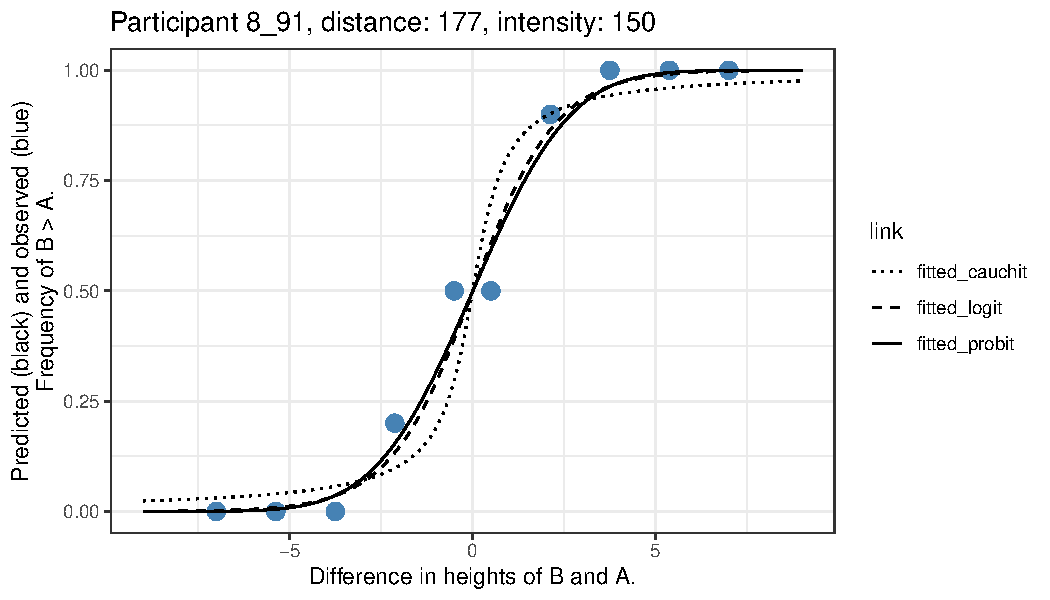
\includegraphics[width=\maxwidth]{figure/id8-91-1} \caption[Logistic regression]{Logistic regression; linetype to be selected}\label{fig:id8-91}
\end{figure}

\end{knitrout}

\begin{knitrout}
\definecolor{shadecolor}{rgb}{0.969, 0.969, 0.969}\color{fgcolor}\begin{figure}
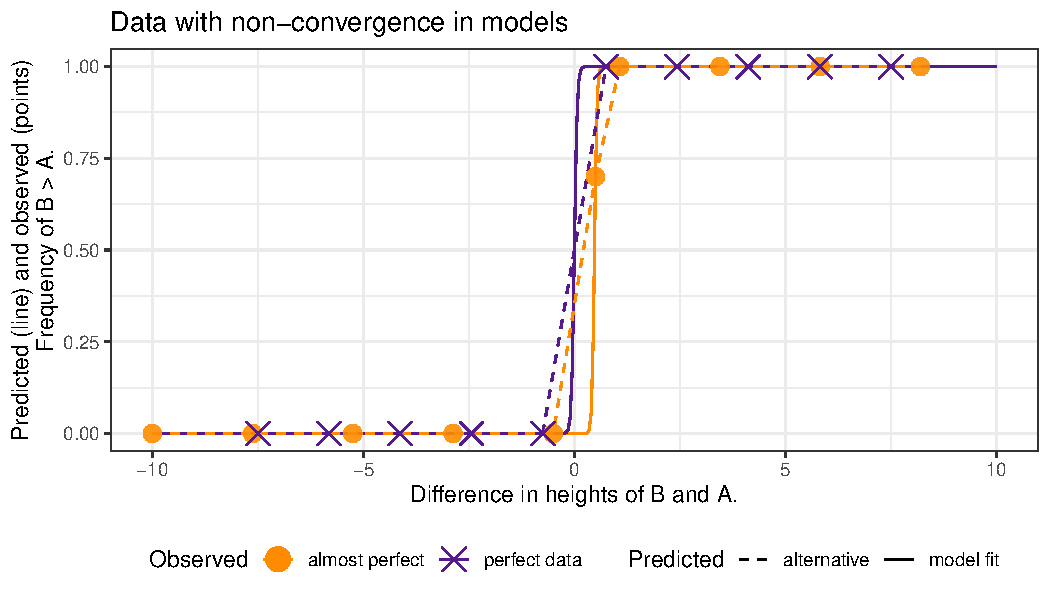
\includegraphics[width=\maxwidth]{figure/lr_problems-1} \caption[Problems with Logistic regressions]{Problems with Logistic regressions}\label{fig:lr_problems}
\end{figure}

\end{knitrout}

\subsection{Two-stage model}

Lu et al fit the data in a two-stage process: 
first, they fit a logistic regression for each participant's data at each level of distance between bars and intensity level. In the example of the barcharts, this fits two parameters (intercept and slope) for each participant for each of the five levels of distance and five levels of intensity for a total of 700 logistic regressions. From these parameters, a participant-level just noticeable difference is calculated as shown in \autoref{jnd.logistic}.

In a second step, these just noticeable differences are then combined in a linear model with covariates of distance and intensity. Lu et al show that log-transforming the dependent variable leads to better model performance. 

Using this modeling approach the resulting model for just noticeable differences shows significant effects for the distance between bars only, while the height of the reference bar does not factor into the model significantly.

Problems with this approach:
Logistic regressions are curious models, in that the convergence of the model fails if the data is ``too good". 
\autoref{fig:lr_problems} shows two examples of potentially observed data that results in the non-convergence of logistic regression as defined in \autoref{mod.logistic}. 
In both cases, the fitted model chooses estimates for the slope that are very high -- alternative models with equally good model fits but far lower slope values are sketched into the figure. 
Changes in the slope directly affect the estimates for the JND values. 
In the example, the estimated slope values change from 30.98 and 36.53 in the fitted models to 2.67 (purple) and 2.54 (orange), respectively. 
This goes in-hand with a ten-fold differences in the associated JND values: the fitted models result in JNDs of 0.04 and 0.03 pixels, respectively, while the alternative fits result in JNDs of 0.41 (purple) and 0.43 pixels (orange).

As a result, the estimated JNDs from the participant-level logistic regressions are more unstable in the case of "too good" data and failed convergence and will thus affect the model fitting at the population level.

Moreover, this two-stage modeling approach introduces extra challenges for variance estimation of the estimated JND in the population-level model. 
Estimating JND at the participant level has variances, and the variance of each estimated JND will be carried on into the population-level model in a complex mathematical form. When the population-level model is fitted, the variance from the participant-level model will be included as part of the variance of the estimated JND at the population level, which not only increases the variance of the population-level JND estimation but also makes it harder to calculate.  





\begin{knitrout}
\definecolor{shadecolor}{rgb}{0.969, 0.969, 0.969}\color{fgcolor}\begin{figure}
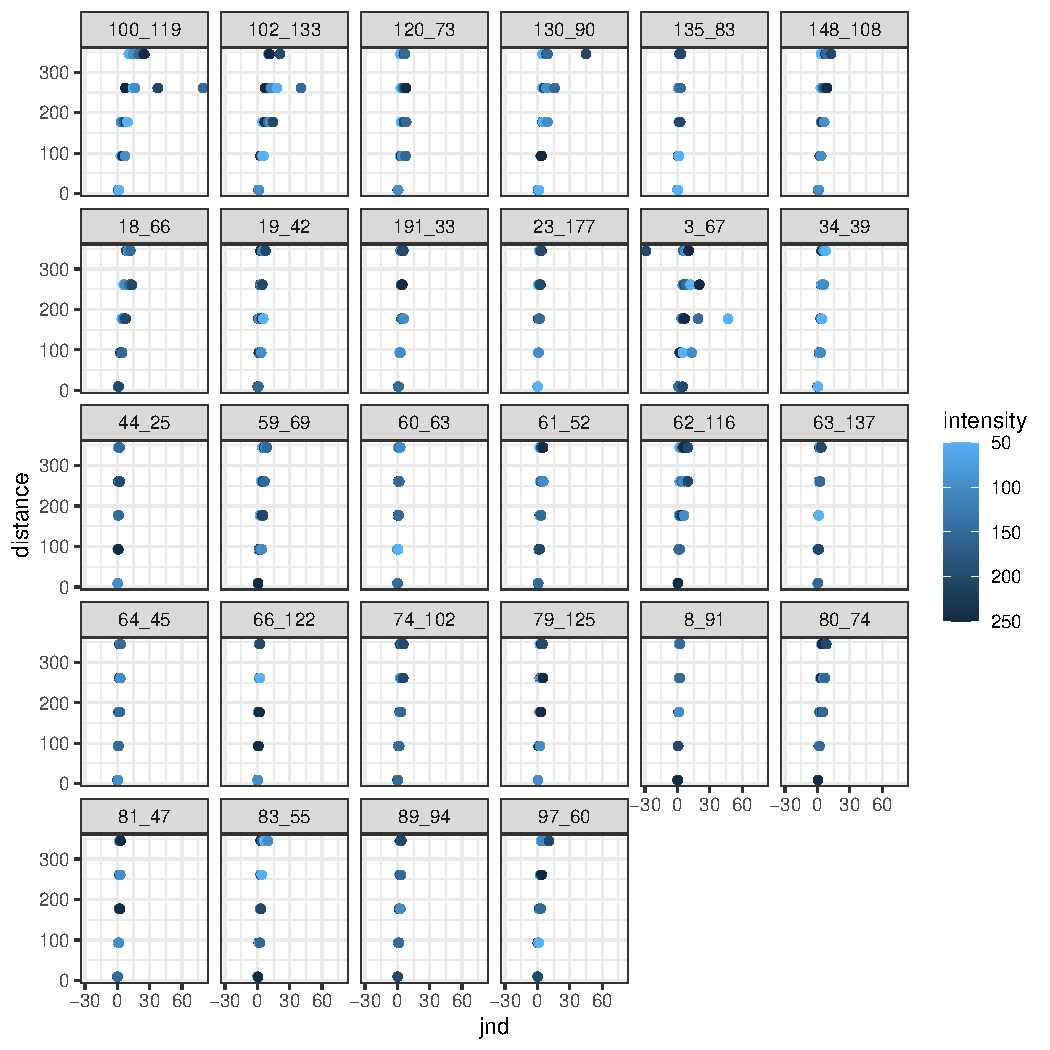
\includegraphics[width=\maxwidth]{figure/jnd_lu-1} \caption[Just noticeable differences for each participant estimated from each participant's data alone]{Just noticeable differences for each participant estimated from each participant's data alone.}\label{fig:jnd_lu}
\end{figure}

\end{knitrout}






\begin{knitrout}
\definecolor{shadecolor}{rgb}{0.969, 0.969, 0.969}\color{fgcolor}\begin{figure}
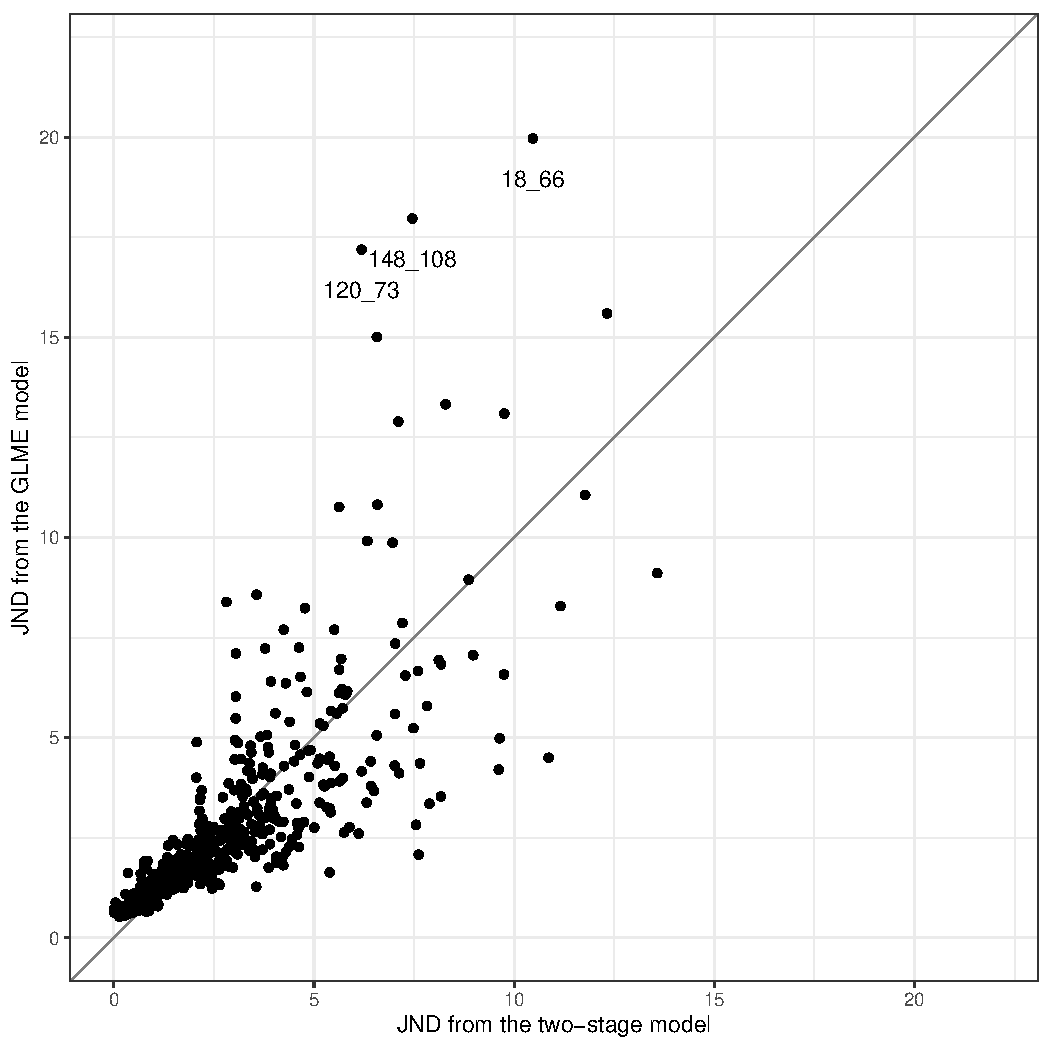
\includegraphics[width=\maxwidth]{figure/models-1} \caption[Scatterplot comparing the JND estimates under Lu's approach and under the approach described here]{Scatterplot comparing the JND estimates under Lu's approach and under the approach described here. The correlation is only 0.75, but most of the values are almost identical. In particular, participant 3\_67 is problematic for the Lu model. Once this participant's values are excluded the correlation between the estimates jumps to 0.98.}\label{fig:models}
\end{figure}

\end{knitrout}


\section{Example: full hierarchical model for JNDs in barcharts}
% Data from Lu et al.; 
We used the bar chart data from Lu at al. \cite{JNDVIS21} to fit a random effects model as shown below: The data set contains $28 \times 5 \times 5 \times 10 = 7000$ observations since we have 28 participants, 5 levels for separation distance, 5 levels for height or intensity of reference bars (A), and 10 levels for height of comparison bars (B). The height difference in pixels between comparison bar B and reference bar A is the signal to be perceived by the participants.

At the population level, model (\autoref{model.bar}) fits three coefficients to estimate the average individual's ability to assess the difference between the heights of two bars A and B. This model depends on: 

\begin{enumerate}
    \item the difference in heights between these two bars (encoded as signal $S$), 
    \item the horizontal distance between bars A and bars B (encoded as distance $D$), and 
    \item the height of bar A (encoded as intensity $I$). Note that bar A is the reference bar with the fixed height in the experiments.
\end{enumerate}

Both distance and intensity are included using a log transform. This transformation improves model performance significantly. It is appropriate given research on human perception of stimuli \cite{logPerception}.

If we extend this model to account for individual effects, we can examine both the population-level trends and the trends for individual participants.
We do this by using random effects. For each participant $j$, $j = 1, ..., 28$, we fit an intercept ($u_{j}$) and an effect in signal size $S$ ($u_{sj}$). 
% and an effect in signal size for neighboring bars ($u_{2j}$).
We make the usual assumptions for random effects of normality and mutual independence, i.e.\ $u_{j} \sim N(0, \sigma_u^2)$ and $u_{sj} \sim N(0, \sigma_s^2)$
% and $u_{d_o} \sim N(0, \sigma_{d_o}^2)$ 
i.i.d. with $u_{j} \perp u_{sj}$ for all $j$ .
% , u \perp u_{d_o},$ and $u_s \perp u_{d_o}$: )
% $u_{0j} \sim N(0, \sigma_0^2)$, $u_{1j} \sim N(0, \sigma_1^2)$, and $u_{2j} \sim N(0, \sigma_{2}^2)$ i.i.d. for all $j$ with $u_{0j} \perp u_{1j}, u_{0j} \perp u_{2j},$ and $u_{1j} \perp u_{2j}$ for all $j$: 

\begin{eqnarray} \nonumber
\label{model.bar}
\text{logit}~P(Y = 1) = \beta_s S &+& \underbrace{\beta_{sd} \log(D) S}_{\text{impact of distance on signal}}  \\ \nonumber
&+& \underbrace{\beta_{si} \log(I) S}_{\text{impact of intensity on signal}} \\ 
&+& \underbrace{u_j + u_{sj} S}_{\text{participants' effects}}
\end{eqnarray}

% \begin{eqnarray} \nonumber
% \text{logit} P(Y = 1) = \beta_s S + \underbrace{\beta_{sd} \log(D) S + \beta_{sd_o} S}_{\text{impact of distance on signal}}  + \\ \label{model.bar}
% \underbrace{\beta_{si} \log(I) S}_{\text{intensity }} +  
% \underbrace{u_j + u_{sj} S + u_{d_oj} S}_{\text{participants' effects}}.
% \end{eqnarray}

% \begin{eqnarray} \nonumber
% \text{logit} P_j(B > A | D, I, S) = \beta_1 S + \underbrace{\beta_{I} \log(I) S}_{\text{intensity }} + \\ \label{model.bar2}
% \underbrace{\beta_{D} \log(D) S + \beta_{N} \I(N = 0) S}_{\text{impact of distance on signal}} +  
% \underbrace{u_{0j} + u_{1j} S + u_{2j} \I(N = 0) S}_{\text{participants' effects}} \\
% = u_{0j} + (\beta_1 + u_{1j} + \beta_{D} \log(D) + \\ \nonumber
% \beta_{I} \log(I) + (\beta_{N} + u_{2j}) \mathbb{I}(N = 0) )S \nonumber.
% \end{eqnarray}

where $S$ is the signal in the study, i.e.\ the difference in heights between bars B and A, i.e.\ if $S$ is negative, bar B is shorter than bar A.
$D$ and $I$ are the distance between the bars and the height of bar A, respectively. 
% $N$, as noted above, is the number of bars between the bars of interest and is used to denote the neighborhood effect.
Note that for the overall population, no intercept is fitted, i.e.\ the point of (relative) subjective equality is set to zero at the population level. Instead, we are interested in how distance and intensity affect a viewer's perception of differences in bars' heights. 

This model is fitted in R using the package \textit{lme4} \cite{lme4} and evaluated using package \textit{lmerTest}\cite{lmerTest}. We have also developed an R Shiny app \cite{shiny} to support users in building GLME models from scratch.

\subsection{The app: Model Buildr}

The Shiny app {\it Model Buildr} assists users in connecting the two-stage modeling approach with the GLME modeling approach. Users can construct their GLME models incrementally, guided by prompts within the app. The process starts with a basic logistic regression for a single participant with one condition level per condition variable. Subsequently, the app extends the logistic regression by incorporating all levels of a chosen condition variable. Users have the option to apply a log transformation to the condition variables and assess the effects of this transformation. These steps aid users in determining the fixed effects to include in the GLME model. Once the fixed effects selection is complete, the app constructs a GLME model by introducing random effects for bias and signal for each participant. The Shiny app {\it Model Buildr} can be accessed at \url{https://csafe.shinyapps.io/Model_Buildr/}


\section{Results}

\begin{table}
\caption{\label{tab:DI} Estimates of fixed effects for the model specified by \autoref{model.bar}.}
\centering

\begin{tabular}{lrrl}
\toprule
Term & Estimate & Std. Error & Pr(>|z|)\\
\midrule
$\beta_s$ & 2.48 & 0.059 & $\le 0.00001$\\
$\beta_{sd}$ & -0.34 & 0.005 & $\le 0.00001$\\
$\beta_{si}$ & -0.04 & 0.005 & $\le 0.00001$\\
\bottomrule
\end{tabular}
\end{table}

\autoref{tab:DI} gives an overview of the fitted estimates for the model specified by \autoref{model.bar} at the population level. All fitted effects are highly significant. 

Model to calculate the just noticeable difference at the population level for a distance between bars of $d$ and a height of the reference bar of $i$. Let $n$ encode the number of bars between the two bars of interest:

\begin{eqnarray}
\label{eq.jnd}
\text{JND}(d, i) &=& 
\frac{\log (3)}{\hat{\beta}_s + \hat{\beta}_{sd} \log(d) + \hat{\beta}_{si} \log(i)} \\ \nonumber
&=&\frac{\log (3)}{2.48 - 0.34 \cdot\log(d) - 0.04 \cdot\log(i)}
\end{eqnarray}




For intensity of 240 pixels of the reference bar, and  distances of $d = 9, 93,$ and 177 between bars, the JNDs will result in \autoref{tb:est_jnd}.

\begin{table}
\caption{\label{tb:est_jnd} Table 2: Estimated JND according to \autoref{eq.jnd}}
\centering
\begin{tabular}{rcr}\hline
JND(9, 240) &=& 0.7293 pixels \\
JND(93, 240) &=& 1.5351 pixels \\
JND(177, 240) &=& 2.2069 pixels\\ \hline
\end{tabular}
\end{table}



With the equation for computing the JND above (\autoref{eq.jnd}), we are able to plot the estimated population-level JND against the variables of interest. \autoref{fig:jnd_intensity_error} plots JND vs intensity given fixed values of distance. What we can see is that when intensity (height of reference bar A) increases, the estimated JND also increases. The 95\% confidence intervals of estimated JND are marked by the ribbon and are calculated using the estimated variance-covariance matrix of fixed effects and the delta method. Note that although the effect of intensity is tiny, it is still significant, and our model with more statistical power is able to capture it. Moreover, increasing the distance between the bars of interest will also increase the estimated JND. 
% And adding the neighborhood effect (when the distance is 9 pixels) can greatly reduce the JND. 
The estimated JNDs for each individual are also plotted in \autoref{fig:jnd_intensity_error}. Note that the spread of individual lines can be considered as a representation of the standard deviation of the individuals, which is different from the standard errors (represented by the confidence intervals) of the model estimates. 
The dashed lines in \autoref{fig:jnd_intensity_error} represent estimated JND values that are extrapolated from the model. Weber's Law builds a proportional relationship between the JND and the initial stimuli intensity \cite{kandel_principles_2013}, and the relationship between the estimated interpolated JND and the intensity (height of reference bar A) can be approximated by a proportional relationship. However, the estimated extrapolated JND does not keep a proportional relationship with the intensity as shown in \autoref{fig:jnd_intensity_error}. This aligns with some research findings that suggest that Weber's Law fails at low intensities \cite{norris_system_1900}.


\begin{knitrout}
\definecolor{shadecolor}{rgb}{0.969, 0.969, 0.969}\color{fgcolor}\begin{figure}
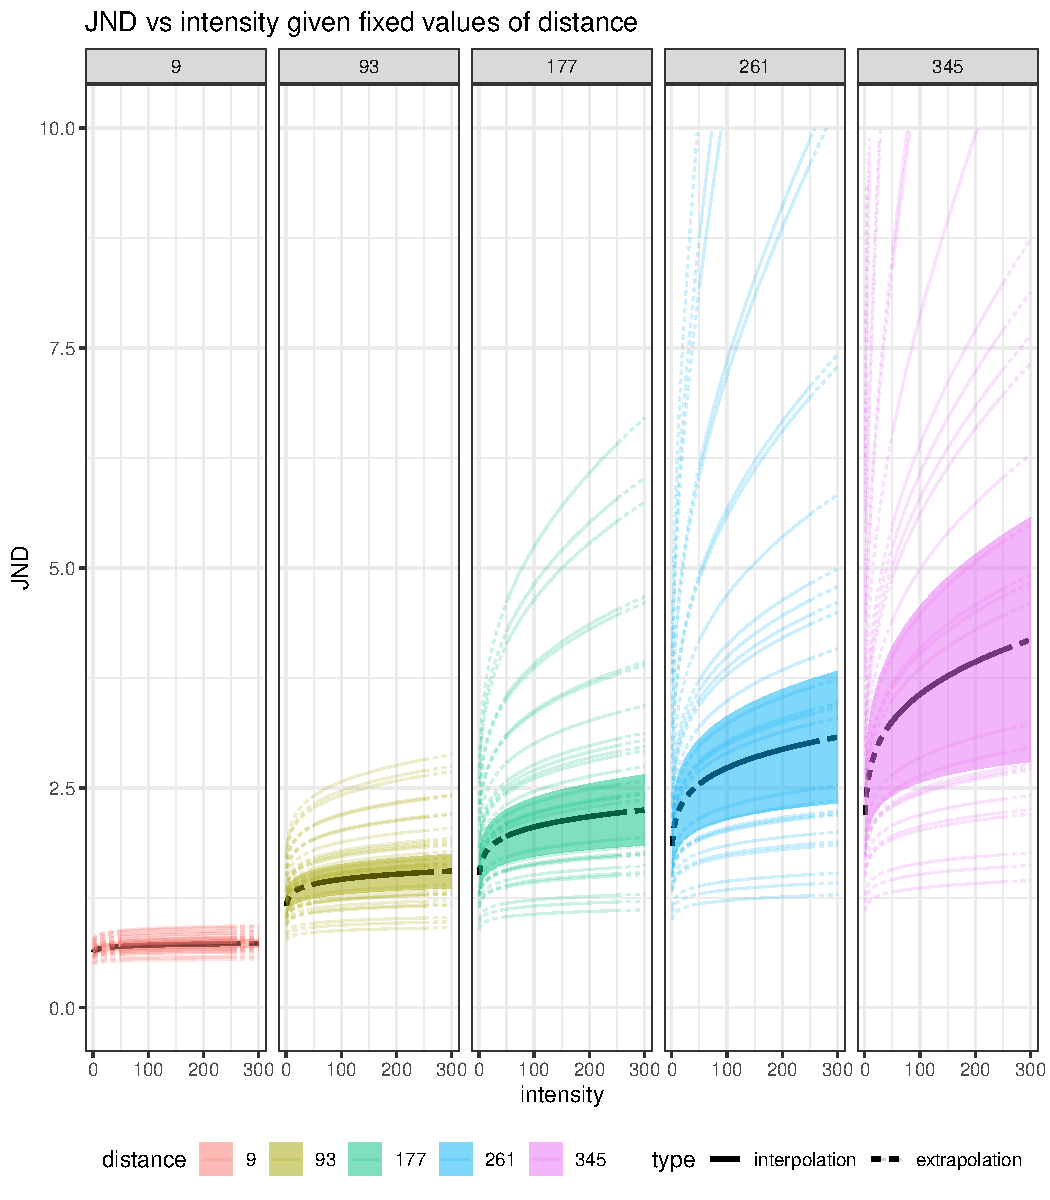
\includegraphics[width=\maxwidth]{figure/jnd_intensity_error-1} \caption[JND vs intensity given fixed values of distance]{JND vs intensity given fixed values of distance. The transparent ribbon area shows the 95\% confidence intervals for the estimated JNDs. The black line is the estimated population-level JNDs, where the solid part and the dashed part are the interpolation and extrapolation of the model, respectively. Other thin lines are the estimated individual-level JNDs. }\label{fig:jnd_intensity_error}
\end{figure}

\end{knitrout}


While the fixed effects in the model specified by \autoref{model.bar} allow us to calculate the JND at the population level, the fitted random effects allow us to inspect the perceptual skill of each participant. Adding the random effects of a participant is essentially adjusting the population-level estimates based on this participant's performance as shown in \autoref{eq:JND_random} and \autoref{fig:pop}. 

\begin{eqnarray}
\label{eq:JND_random}
\text{JND}(d, i, j) = \frac{\log (3)}{(\hat{\beta}_s + \hat{u}_{sj}) + \hat{\beta}_{sd} \log(d) + \hat{\beta}_{si} \log(i) }
\end{eqnarray}


\begin{knitrout}
\definecolor{shadecolor}{rgb}{0.969, 0.969, 0.969}\color{fgcolor}\begin{figure}
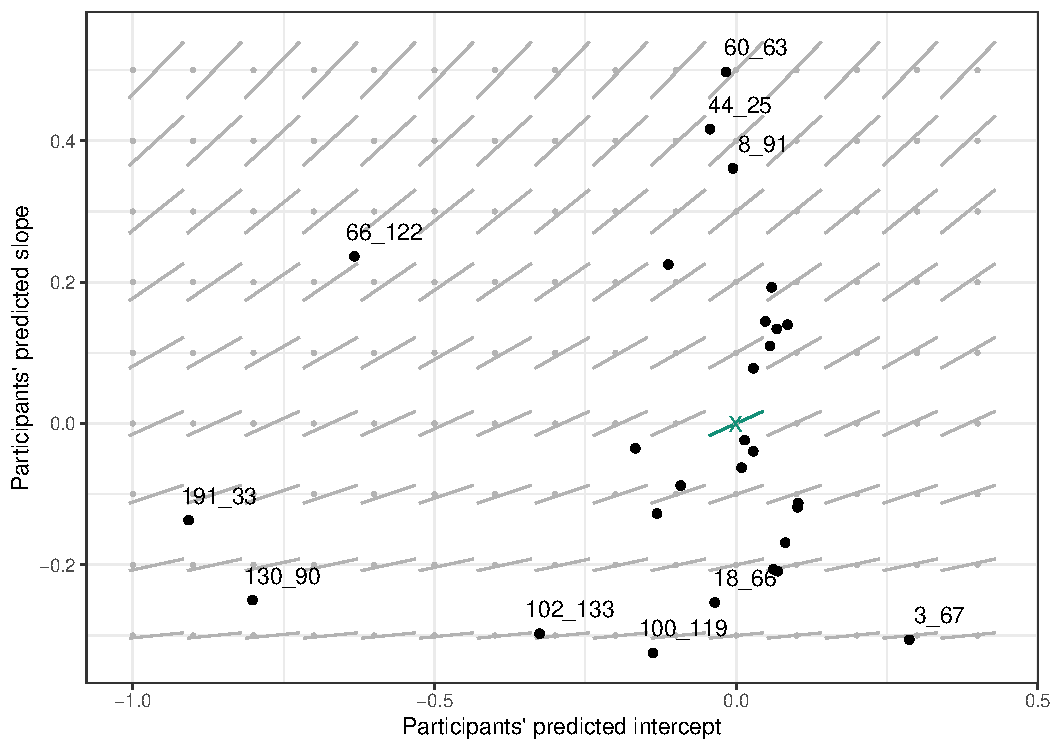
\includegraphics[width=\maxwidth]{figure/ranef-bar-1} \caption[Overview of participant-based predictions]{Overview of participant-based predictions. The green cross indicates the overall population based average. The further away a participant appears on the scatterplot, the more distinctly different their answers are from the population average. The faint grey line segments indicate how the random effects model a participant's perception. }\label{fig:ranef-bar}
\end{figure}

\end{knitrout}

\autoref{fig:ranef-bar} gives an overview of the participant-specific effects. 
Participants' perceptual skills can be measured directly from the ordering along the slope variable: because the Just Noticeable Difference is inversely proportional to the slope of the estimated probability curve along the signal, the only difference in the JND of two participants $j_1$ and $j_2$ is their predicted slope values $\hat{u}_{sj_1}$ and $\hat{u}_{sj_2}$.

The light grey line segments and dots in \autoref{fig:ranef-bar} are intended to provide a reference on how the random effects in the model account for individuals' perceptual skills. All line segments are shown with respect to the overall population average (shown in green). An increase in slope indicates that a participant is able to spot smaller differences between the bars' heights. 
The dot next to the line segment serves as a point of reference to the theoretical point of equilibrium (0, 0.5). When the line segment is moving away from this point of reference, it means that a participant is exhibiting a subjective bias: when the reference point is on the left of the line segment,  a participant has a tendency to respond that B is not larger than A. Three participants (68-122, 191-33, and 130-90) show a strong bias in this direction. Participant 3-67 exhibits the strongest bias in the other direction, i.e.\ has a tendency to respond that B is larger than A.

Responses from individuals labeled in \autoref{fig:ranef-bar} are shown in \autoref{fig:individuals}. 

\begin{knitrout}
\definecolor{shadecolor}{rgb}{0.969, 0.969, 0.969}\color{fgcolor}\begin{figure}
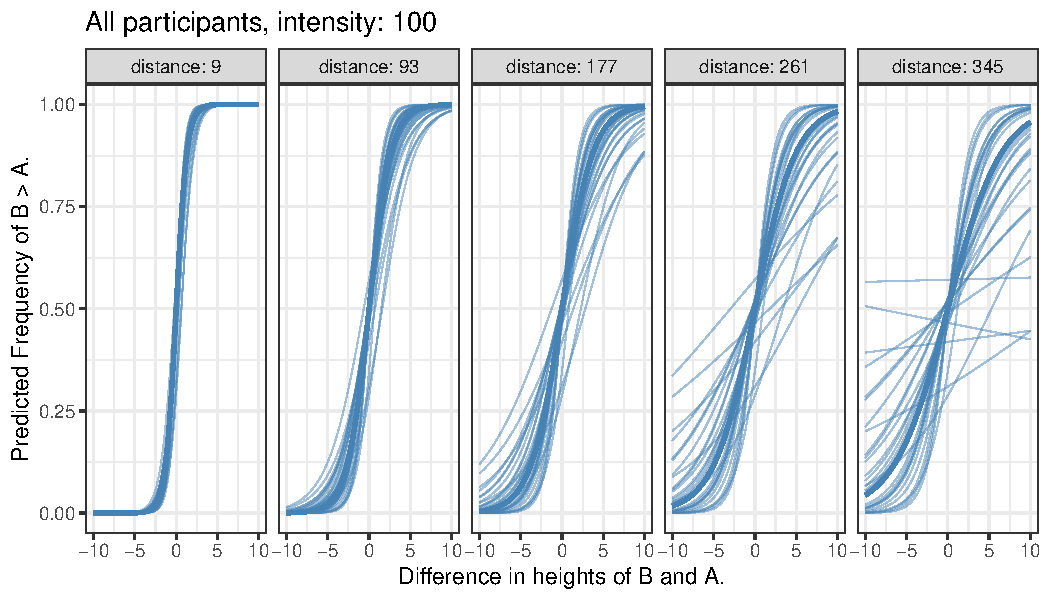
\includegraphics[width=\maxwidth]{figure/pop-1} \caption[Predictions for overall population (thick lines) and each of the participants (thin lines)]{Predictions for overall population (thick lines) and each of the participants (thin lines)}\label{fig:pop}
\end{figure}

\end{knitrout}





\begin{knitrout}
\definecolor{shadecolor}{rgb}{0.969, 0.969, 0.969}\color{fgcolor}\begin{figure}
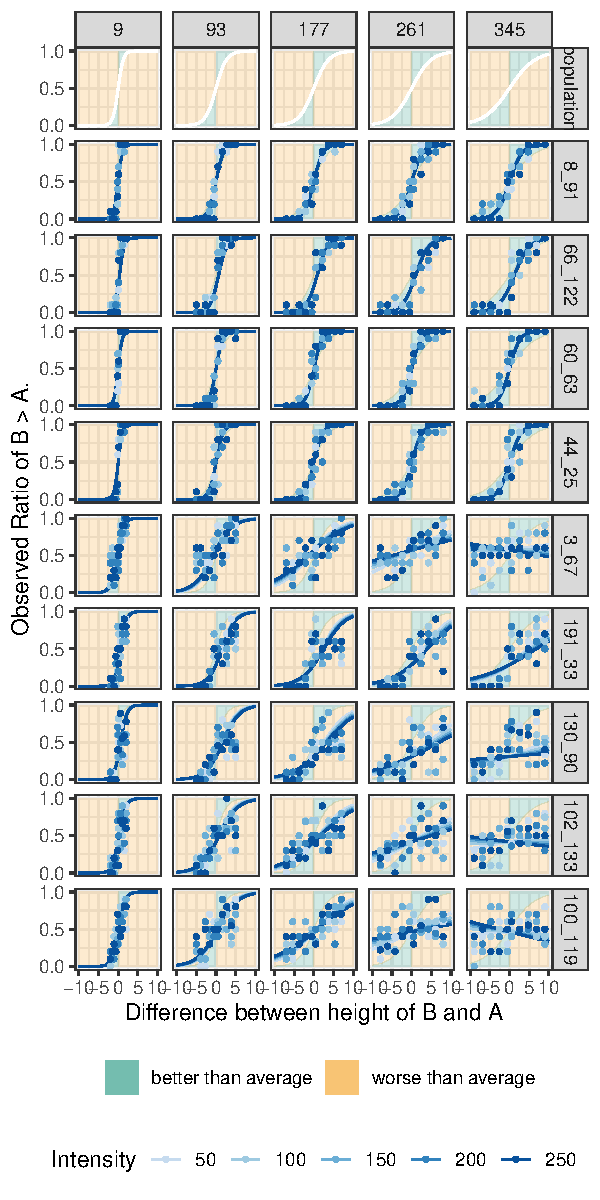
\includegraphics[width=\linewidth]{figure/individuals-1} \caption[Overview of  participants with the most extreme values in subject-specific skill (slope) and intercept (PSE away from zero)]{Overview of  participants with the most extreme values in subject-specific skill (slope) and intercept (PSE away from zero).}\label{fig:individuals}
\end{figure}

\end{knitrout}

\autoref{fig:residuals}(a) is the ``residuals vs fitted values" plot for the model specified by \autoref{model.bar}. The grouping structure is seemingly worrying but is actually expected. It is caused by the discrete levels of intensity, distance, and participants. To see how the discrete nature of these variables leads to the structure in the residual plot, we simulate binomial samples for each combination of intensity, distance, participants, and signal values based on the fitted probabilities of model (\autoref{model.bar}). Then the simulated data is used to fit a model with the same model structure as model (\autoref{model.bar}), and its residual plot is shown as \autoref{fig:residuals}(b). The original data of \cite{JNDVIS21} reveal that some combinations of intensity, distance, participants, and signal values do not have exactly 10 trials, but the simulated data are sampled with fixed 10 trials for each combination. This difference results in the fact that every point in \autoref{fig:residuals}(b) can fit in one of the diagonal structures. And we can see from the comparison of the two residual plots that the diagonal structure is caused by the discrete nature of the variables. 

In \autoref{fig:model_compare_plot}, the fitness of the GLME approach and the two-stage approach is compared at the population level. The red dots represent the average probability of predicting that the comparison bar is higher for the 28 participants across all combinations of intensity and distance. And the grey dots represent the probabilities of each individual. The population-level predictions are made by the fixed effects of the GLME model (solid lines) and the second-stage model of the two-stage model (dashed lines). 

What we see from our comparisons between the GLME approach and the two-stage approach is that the two-stage model can better fit the data at the individual level. The reasoning behind this lies in the structural design of these models: the two-stage approach fits a logistic regression model for each combination of distance, intensity, and individual, while the GLME approach pulls information across various individuals when making individual-level predictions. However, \autoref{fig:model_compare_plot} shows that the GLME model is more effective in capturing the population-level trend for most combinations of the two variables, which aligns with the core objective of the study and allows for broad generalization.

% Note: Lu's model, better for fitting individual data; our model pulls information from other individuals. At the population level, our model is better in capturing the overall trend
% population level is more important since that is what the study cares about in the first place (results/conclusions can be generalized)
% Lu's model cannot handle participants with negative estimated jnd?
% compute mse?

\begin{knitrout}
\definecolor{shadecolor}{rgb}{0.969, 0.969, 0.969}\color{fgcolor}\begin{figure}
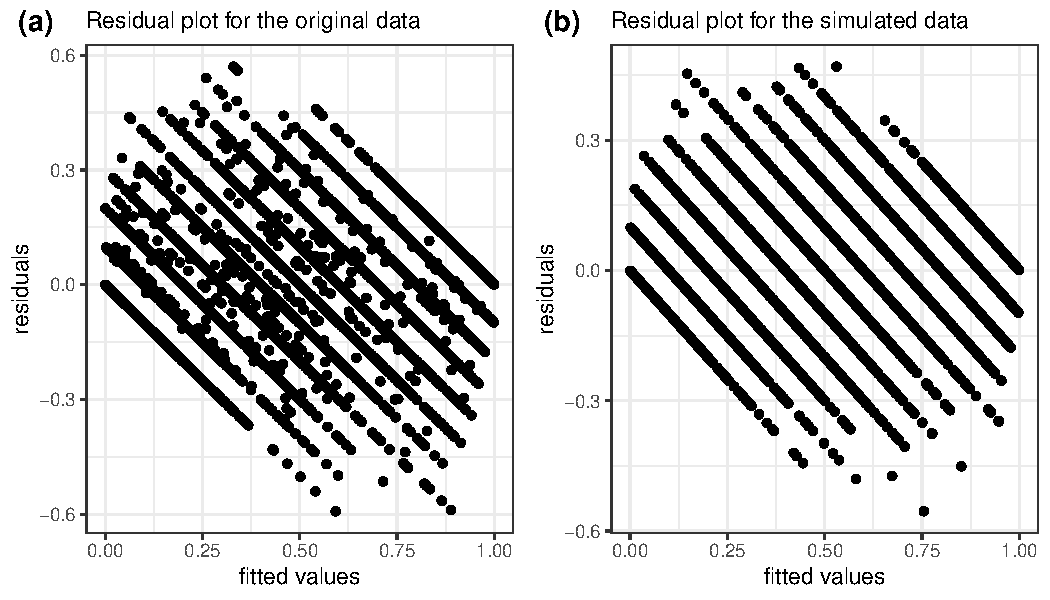
\includegraphics[width=\linewidth]{figure/residuals-1} \caption[(a) Residual plot for the original data and our proposed model]{(a) Residual plot for the original data and our proposed model. (b) Residual plot for the simulated data and our proposed model. The simulated data are binomial samples with fixed 10 trials and fitted probability for each combination of intensity, distance, participants, and signal values. The comparison of the two residual plots show that the diagonal structures presented in the residual plots are actually expected and are caused by the discrete nature of the variables.}\label{fig:residuals}
\end{figure}

\end{knitrout}



\begin{knitrout}
\definecolor{shadecolor}{rgb}{0.969, 0.969, 0.969}\color{fgcolor}\begin{figure}
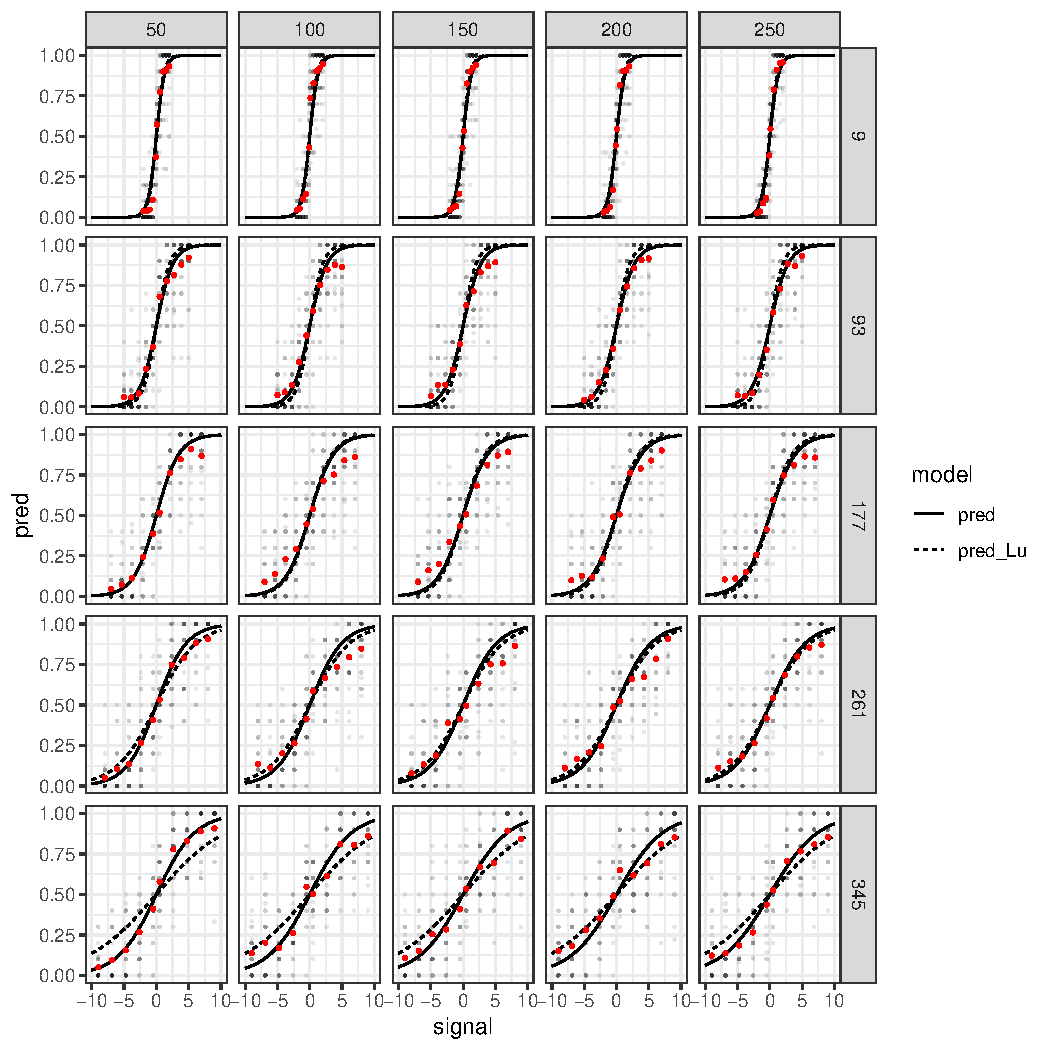
\includegraphics[width=\maxwidth]{figure/model_compare_plot-1} \caption[Comparison of the fitness of the GLME approach and the two-stage approach at the population level]{Comparison of the fitness of the GLME approach and the two-stage approach at the population level. The red dots show the average prediction results of the 28 participants. The fitted population-level curves of the GLME approach and the two-stage approach are presented with solid lines and dashed lines, respectively.}\label{fig:model_compare_plot}
\end{figure}

\end{knitrout}


\section{Discussion}

In this paper, we demonstrate the advantages of modeling psychophysical data using a generalized linear mixed-effect model (GLMM). The two-stage modeling approach is widely used in the field of psychophysics and is taken by Lu et al.\ \cite{JNDVIS21}. This approach fits individual-level models first and then builds a single population-level model based on the individual effects. We show that a mixed-effect model provides more benefits than fitting a two-stage model. A mixed-effect model considers individual-level effects as random effects and population-level effects as fixed effects and incorporates both in one single model, which provides more statistical power and better interpretability.

We also developed a shiny app called \textit{Model Buildr}, which makes it easier for researchers to identify the model, the variables, and the cognitive settings and apply the mixed-effect method to their own topics. This shiny app captures lots of datasets and can be used for many other similar studies.

The data set we used here is from \cite{JNDVIS21}. Using the two-stage approach, Lu et al. \cite{JNDVIS21} fitted a logistic regression to compute a JND for each combination of distance, intensity and participant, and then used the estimated JND as the response variable to build a population-level model.
Using the mixed-effect model approach, we can include and analyze both population-level and individual-level effects in just one model.  

Lu et al. did not find the effect of intensity significant with the two-stage modeling approach. And log-transformation of JND was needed at the population-level model to stabilize the variance. 
With more statistical power, the mixed-effect model does find the effect of intensity tiny but significant. Log-transformation was applied to variables intensity and distance to align with research on human perception of stimuli \cite{logPerception}.

Note that in the original experimental design of \cite{JNDVIS21}, the ranges of signal values are the same across different intensity levels for each distance level. But for each intensity level, the ranges of signal values increase as the distance increases. This means that, for a fixed intensity level, more signals are presented to participants as the distance increases; however, for a fixed distance level, the amount of signals in pixels remains the same across different intensity levels. This design conceals the effect of intensity, especially for the participants who are not good at the task.
For example, participant ``100\_119" in \autoref{fig:individuals} was not able to properly spot the difference in height for bar A and B with the current experimental setup when the distance is 345 pixels. The range of signals should have been enlarged to a point where even participants not good at the task can spot the difference. Since the effect of intensity is potentially concealed by the setup, a model with more statistical power is needed in order to find the significant effect of intensity.

Moreover, the mixed-effect model provides better interpretability. For example, if the distance between bar A and bar B increases from 100 pixels to 200 pixels, the task of determining the higher bar becomes more difficult. As a result, the estimated population-level JND increases, and the slope of the predicted probability curve decreases by approximately 0.1554 ($\hat{\beta}_D (\log(200) - \log(100))$). The decrease of the slope can then be translated into the following statement: on average when bar B is one pixel higher than bar A, the odds of predicting bar B is higher will decrease by 14.39\% ($1 - 1 / \exp(0.1554)$) if the distance between the two bars increases from 100 pixels to 200 pixels.

The following formula calculates the change of JND:
\begin{equation}
    \frac{\log(3)}{\beta} - \frac{\log(3)}{\beta + c} = \frac{\log(3)}{\beta} \frac{c}{\beta + c}
\end{equation}

We really appreciate the efforts of Lu et al. \cite{JNDVIS21} for making their work open source. These efforts of Lu et al. and other researchers make the discussion about various methods and potential improvements possible. We emphasize the importance of open science since it promotes reproducibility of the work, accessibility for the public, and collaboration for future research. It allows researchers to share their insights, collaborate, and build upon each other's work.
Our work is publicly available at: \url{https://github.com/willju-wangqian/one_model_that_fits_them_all}
The world of open science will be constructed by more and more such efforts and contributions from the community.


\appendices
% \section{Psychometric Functions}
% \subsection{Logistic}

% \subsection{Power Law}

% \subsection{Cyclic Power Law}


\section{Error Estimates}

First stage regression: $$\frac{\log{p_{ij\cdot\cdot m}}}{1-\log{p_{ij\cdot\cdot m}}} = \beta_{0ijm} + \beta_{1ijm} x_{ijklm} + \epsilon_{ijklm}$$

Typically, it is assumed that $\epsilon_{ijklm} \sim N(0, \sigma)$.

As a result of this modeling process, $\beta_{1ijm}$ is a random variable (because it is a function of the random variables $x_{ijklm}$ and $y_{ijklm}$). The variance of $\beta_{1ijm}$ can be calculated using Fisher's information matrix, but that calculation is ancillary to the primary goal here, which is to trace the errors from the first stage regression to the next stage. 

The JND calculated for each condition (separation distance $i$ and intensity $j$) and participant $m$ is a function of $\beta_{1ijm}$: $$JND_{ijm} = \frac{\log 3}{\beta_{1ijm}}.$$ 
By the delta method, we can calculate the variance of the JND as $$\text{Var} (JND) = \left(\frac{\log 3}{\beta_{1ijm}^2}\right)^2 \text{Var}\beta_{1ijm}$$. 

% you can choose not to have a title for an appendix
% if you want by leaving the argument blank
% \section{}
% Appendix two text goes here.


% use section* for acknowledgment
\ifCLASSOPTIONcompsoc
% The Computer Society usually uses the plural form
\section*{Acknowledgments}
\else
% regular IEEE prefers the singular form
\section*{Acknowledgment}
\fi


The authors would like to thank...


% Can use something like this to put references on a page
% by themselves when using endfloat and the captionsoff option.
% \ifCLASSOPTIONcaptionsoff
%   \newpage
% \fi



% trigger a \newpage just before the given reference
% number - used to balance the columns on the last page
% adjust value as needed - may need to be readjusted if
% the document is modified later
%\IEEEtriggeratref{8}
% The "triggered" command can be changed if desired:
%\IEEEtriggercmd{\enlargethispage{-5in}}

% references section

% can use a bibliography generated by BibTeX as a .bbl file
% BibTeX documentation can be easily obtained at:
% http://mirror.ctan.org/biblio/bibtex/contrib/doc/
% The IEEEtran BibTeX style support page is at:
% http://www.michaelshell.org/tex/ieeetran/bibtex/
\bibliographystyle{IEEEtran}
\bibliography{references.bib}


% biography section
% 
% If you have an EPS/PDF photo (graphicx package needed) extra braces are
% needed around the contents of the optional argument to biography to prevent
% the LaTeX parser from getting confused when it sees the complicated
% \includegraphics command within an optional argument. (You could create
% your own custom macro containing the \includegraphics command to make things
% simpler here.)
%\begin{IEEEbiography}[{\includegraphics[width=1in,height=1.25in,clip,keepaspectratio]{mshell}}]{Michael Shell}
% or if you just want to reserve a space for a photo:

% \begin{IEEEbiography}{Michael Shell}
% Biography text here.
% \end{IEEEbiography}
% 
% % if you will not have a photo at all:
% \begin{IEEEbiographynophoto}{John Doe}
% Biography text here.
% \end{IEEEbiographynophoto}

% insert where needed to balance the two columns on the last page with
% biographies
%\newpage

% \begin{IEEEbiographynophoto}{Jane Doe}
% Biography text here.
% \end{IEEEbiographynophoto}

% You can push biographies down or up by placing
% a \vfill before or after them. The appropriate
% use of \vfill depends on what kind of text is
% on the last page and whether or not the columns
% are being equalized.

%\vfill

% Can be used to pull up biographies so that the bottom of the last one
% is flush with the other column.
%\enlargethispage{-5in}



% \section{Conclusion}
% The conclusion goes here.


% that's all folks
\end{document}

